% Generated from the Notion page by tools/notion2tex.py (see report/README.md).
\section{Final Architecture}\label{sec:4}

The selected design is the one carried through all four verification steps: C17 (C simulation and HLS synthesis), C20 (C/RTL co-simulation) and C22 (Vivado place and route at 5 ns). Its source was produced by the agent over 200+ experiments. For reading, we had the agent rewrite it as a plain version with the macros substituted and the templates expanded, and re-ran C simulation and synthesis on both: the outputs are bit-identical and the synthesis results are the same.

The readable version is reproduced in Appendix~\ref{app:code-readable}; the original source is \path{designs/winograd_t4_windows32_v1/srcnn.cpp} in the project repository.

However, even so, we must mention that, for the agent optimization are extreme detailed, this chapter does not walk through the code. It explains the design one decision at a time: what constraint forced the decision, which experiment measured the alternatives, and what the chosen structure costs.

\subsection{Dataflow}\label{sec:4.1}

At the top level the design is organised by function, which gives a direct view of the dataflow.  The baseline was slow for a structural reason: inside each 16$\times$16 tile the three layers run one after another, every tile re-fetches a 28$\times$28 input window from DDR to produce 16$\times$16 outputs, the weights are reloaded over AXI on every call, and only 3.69 \% of the DSPs are ever busy. We wanted the opposite: keep everything the network produces on the chip, use no external scratch buffer at all (the one attempt with DDR scratch buffers, S01, was abandoned), and let the three layers work at the same time on different pixels. Task-level dataflow with \texttt{hls::stream} connections between the stages gives both at once.

The open question is how much to buffer between stages. Holding the full outputs of Conv1 and Conv2 (255$\times$255$\times$64 and 255$\times$255$\times$32 values) takes 23.81 MiB in float, while the device offers 5.1 Mb of BRAM and 18 Mb of URAM, about 2.9 MiB in total; even at 8 bits the two maps would not fit. So, neighbouring stages exchange single pixels (one pixel's channel vector), and only a stage that needs a spatial neighbourhood keeps a line buffer of a few rows, even more, every FIFO in the design has an explicitly chosen depth. Figure~\ref{fig:3} shows the resulting top-level structure.

\begin{figure}[!htbp]
\centering
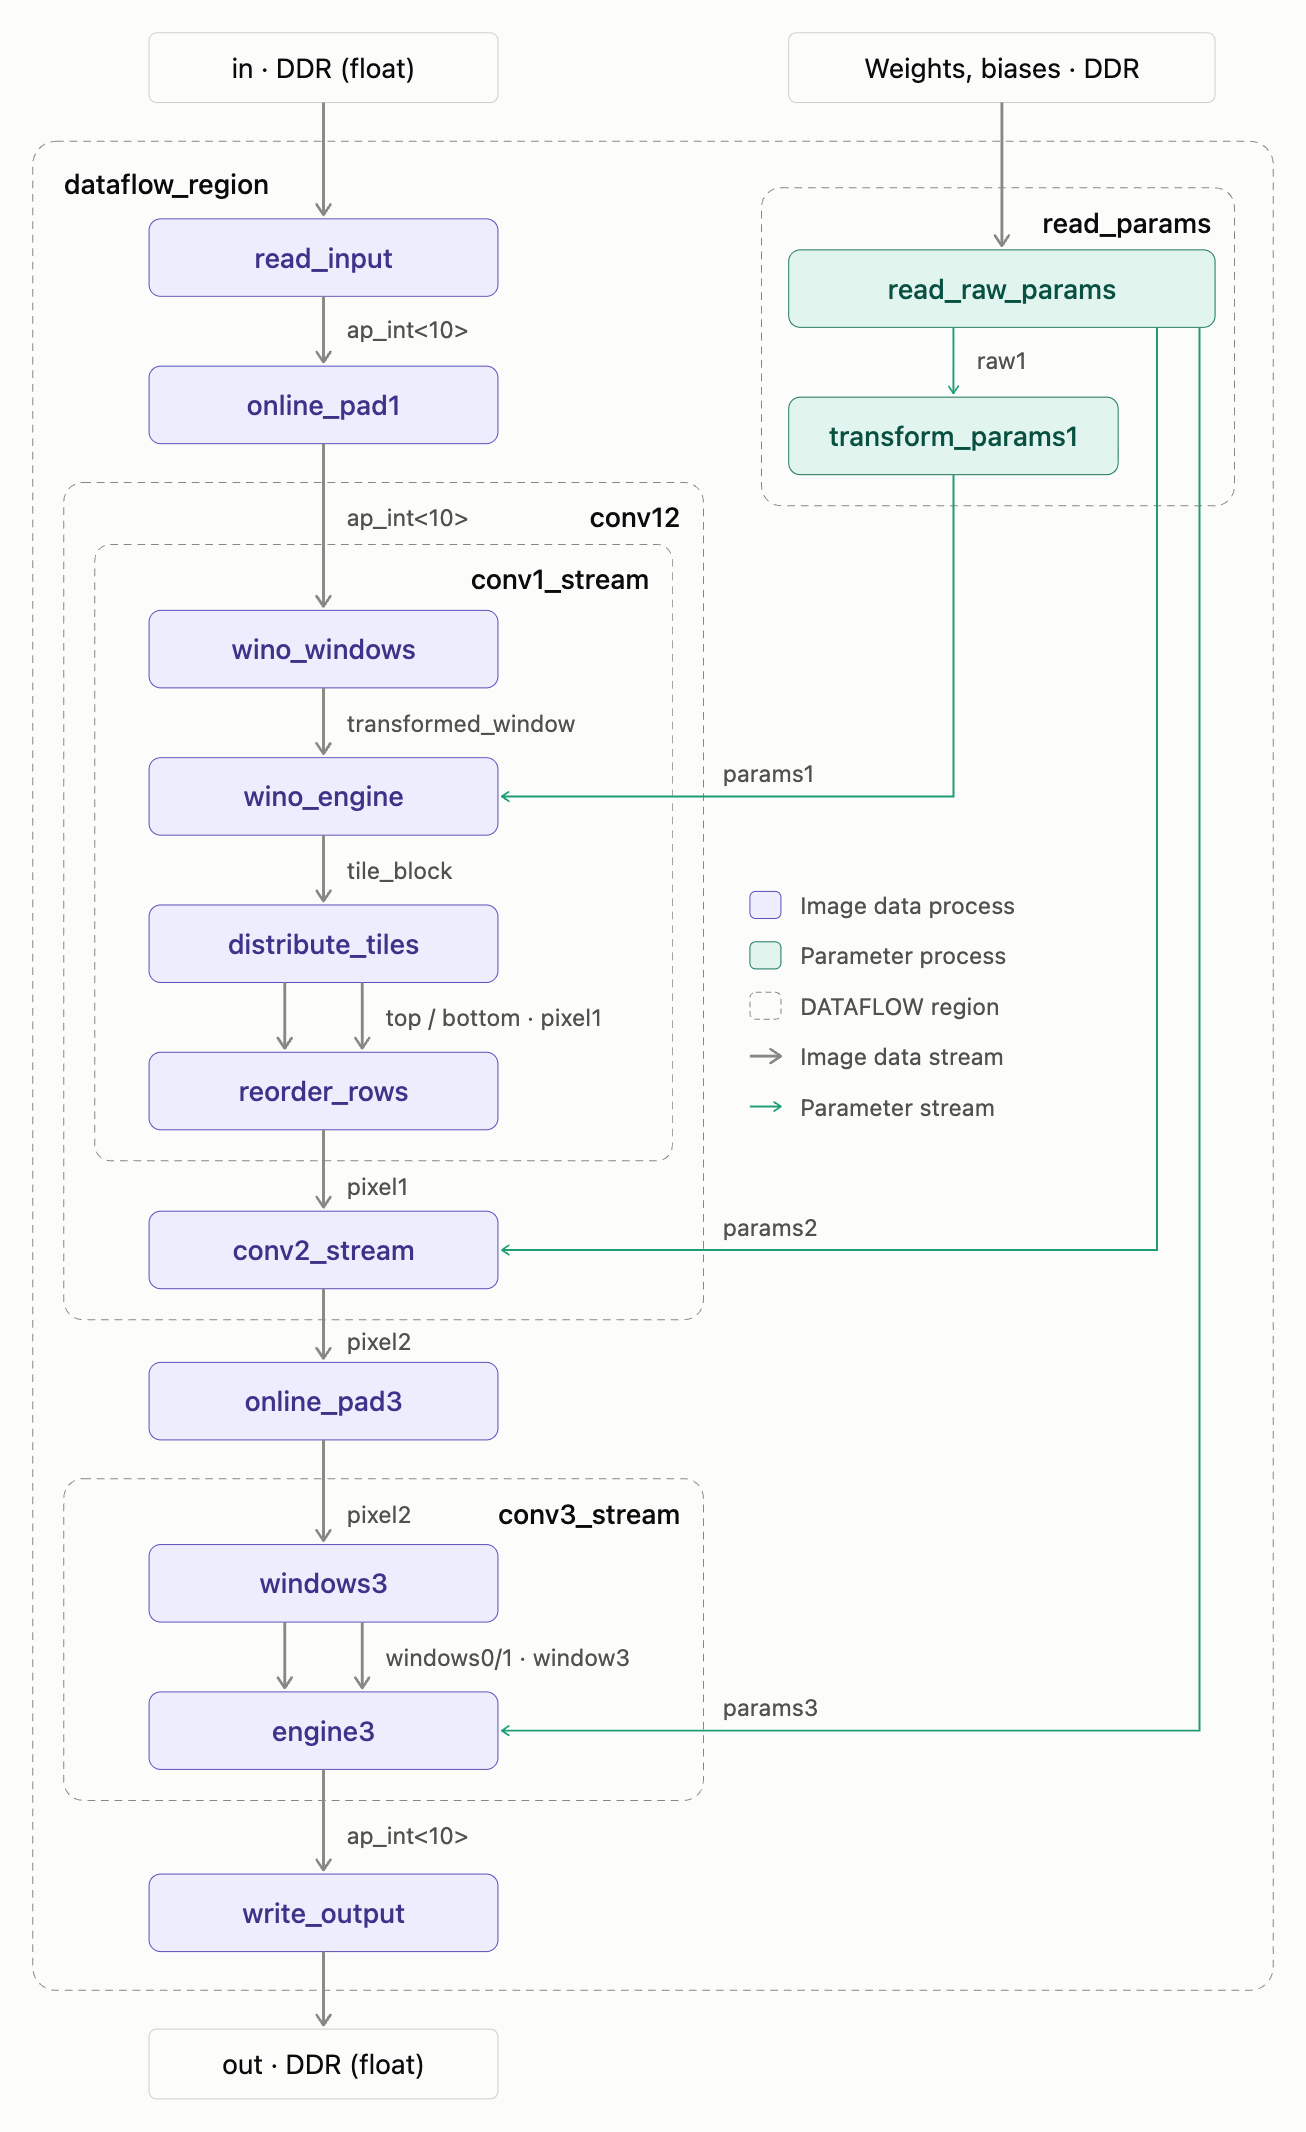
\includegraphics[width=0.72\linewidth,height=0.48\textheight,keepaspectratio]{figures/fig03-top-level-structure.png}
\caption{Top-level structure of the selected design: the dataflow region with its image-data processes (purple) and parameter processes (green), the nested DATAFLOW regions conv12, conv1\_stream and conv3\_stream, and the stream type passed between each pair of stages. Weights are read from DDR and transformed once per frame, then streamed to the three engines.}
\label{fig:3}
\end{figure}

\begin{table}[!htbp]
\centering
\scriptsize
\caption{Stages of the dataflow region of the selected design (C17), in data order: the element each stage passes on and its width, the FIFO depth, the on-chip memory it keeps (routed, C22), the loop trip count per frame from the source, and the active cycles and stall share measured in C/RTL co-simulation C20.}
\label{tab:3}
\begin{tabularx}{\linewidth}{lYR{0.9cm}R{1.3cm}YR{1.4cm}R{1.6cm}R{1.0cm}}
\toprule
Stage & Input $\rightarrow$ output element & Width (bits) & FIFO depth (out) & Internal memory & Iterations per frame (design) & Iterations per frame (C/RTL co-simulation) & Stall Percent \\
\midrule
\texttt{read\_input} & float from DDR $\rightarrow$ pixel \texttt{ap\_int<10>} & 10 & 512 & none & 65,025 & 78,653 & 66.9 \% \\
\texttt{online\_pad1} & pixel $\rightarrow$ pixel, 255\textsuperscript{2} $\rightarrow$ 264\textsuperscript{2} replicate-padded & 10 & 16 & 1 row, 255 $\times$ 10 b (1 BRAM18K) & 69,696 & 69,962 & 72.9 \% \\
\texttt{wino\_windows} & pixel $\rightarrow$ transformed window, 9 sub-blocks $\times$ 16 $\times$ \texttt{ap\_int<12>} & 1,728 & 32 (LUTRAM) & 9 rows $\times$ 264 $\times$ 10 b (9 BRAM18K) + 10$\times$10 window registers & 69,696 & 69,699 & 73.1 \% \\
\texttt{wino\_engine} & window $\rightarrow$ tile, 2$\times$2 pixels $\times$ 64 ch $\times$ 10 b & 2,560 & 2 (LUTRAM) & transformed weights 64 $\times$ 9 $\times$ 16 $\times$ 14 b = 129 kb (LUTRAM) & 262,144 & \textbf{262,924} & \textbf{2.5 \%} \\
\texttt{distribute\_tiles} & tile $\rightarrow$ 2 pixel streams (\texttt{top}, \texttt{bottom}), 64 ch $\times$ 10 b & 640 & 512 each (BRAM, 18 BRAM18K each) & none & 65,536 & 65,537 & 74.8 \% \\
\texttt{reorder\_rows} & 2 streams $\rightarrow$ raster-order pixel, 64 ch & 640 & 4 & none & 65,025 & 65,026 & 75.4 \% \\
\texttt{conv2\_stream} & 64-ch pixel $\rightarrow$ 32-ch pixel & 320 & 4 & packed weights 16 $\times$ 64 $\times$ 27 b = 27.6 kb (LUTRAM) & 260,100 & \textbf{262,275} & \textbf{3.2 \%} \\
\texttt{online\_pad3} & pixel $\rightarrow$ pixel, 255\textsuperscript{2} $\rightarrow$ 259\textsuperscript{2} padded & 320 & 16 & 1 row, 255 $\times$ 320 b (9 BRAM18K) & 67,081 & 67,347 & 75.3 \% \\
\texttt{windows3} & pixel $\rightarrow$ two half windows, 25 taps $\times$ 16 ch $\times$ 10 b each & 4,000 + 4,000 & 2 + 2 & 4 rows $\times$ 259 $\times$ 320 b (36 BRAM18K) + 5$\times$5$\times$32 window registers & 67,081 & 67,084 & 75.4 \% \\
\texttt{engine3} & two half windows $\rightarrow$ output pixel & 10 & 16 & weights 32 $\times$ 25 $\times$ 10 b = 8 kb (LUTRAM) & 260,100 & \textbf{260,977} & \textbf{4.4 \%} \\
\texttt{write\_output} & pixel $\rightarrow$ float to DDR & 32 & -- & none & 65,025 & 65,042 & 76.2 \% \\
\texttt{read\_params} $\rightarrow$ \texttt{transform\_params1} & 8,129 floats $\rightarrow$ three parameter streams & 224 / 10 / 10 & 4 / 16 / 16 & raw 9$\times$9 kernel registers & 8,129 + 640 & 10,487 / 7,234 & 0.2 \% / 1.4 \% \\
\bottomrule
\end{tabularx}
\end{table}

Table~\ref{tab:3} lists every process for one frame in the dataflow region with the shape and width of the element it passes on, the FIFO depth, the memory it keeps internally, and two numbers about time. \emph{Iterations per frame (design)} is the loop trip count read from the source: for a loop with II = 1 it is the number of cycles the stage needs when it is never blocked, so it is a lower bound, not a measurement. \emph{Iterations per frame (C/RTL co-simulation)} is measured after Vitis C/RTL co-simulation: from the latency of the process within one frame (\texttt{process\_latency\_avg\_cycles}, up to 273,052 cycles) we subtract \texttt{read\_stall\_cycles} and \texttt{write\_stall\_cycles}, which gives the number of cycles in which the stage was actually processing data. \emph{Stall Percent} is the share of the frame in which the process waited on a FIFO (\texttt{stall\_pct}).

Whether a dataflow pipeline is actually balanced can only be seen in C/RTL co-simulation, where every FIFO and process is instrumented. Figure~\ref{fig:4} shows the measured blocking of each FIFO over two RTL frames: the three engines (wino\_engine, conv2\_stream, engine3) wait less than 5 \% of the time, while every producer in front of them is write-blocked about 73 \% of the time and every consumer behind them is read-blocked about 75 \% of the time. This is the expected signature of a pipeline whose throughput is set by the compute engines rather than by the data movement. The inset records the one FIFO change that mattered: raising the window FIFO from depth 2 (C13/C14) to depth 32 (C17/C20) removed 58,166 read-block cycles from the Winograd fold loop and brought the frame from 300,632 to 273,023 cycles (1.503 ms to 1.365 ms at 5 ns).

\begin{figure}[!htbp]
\centering
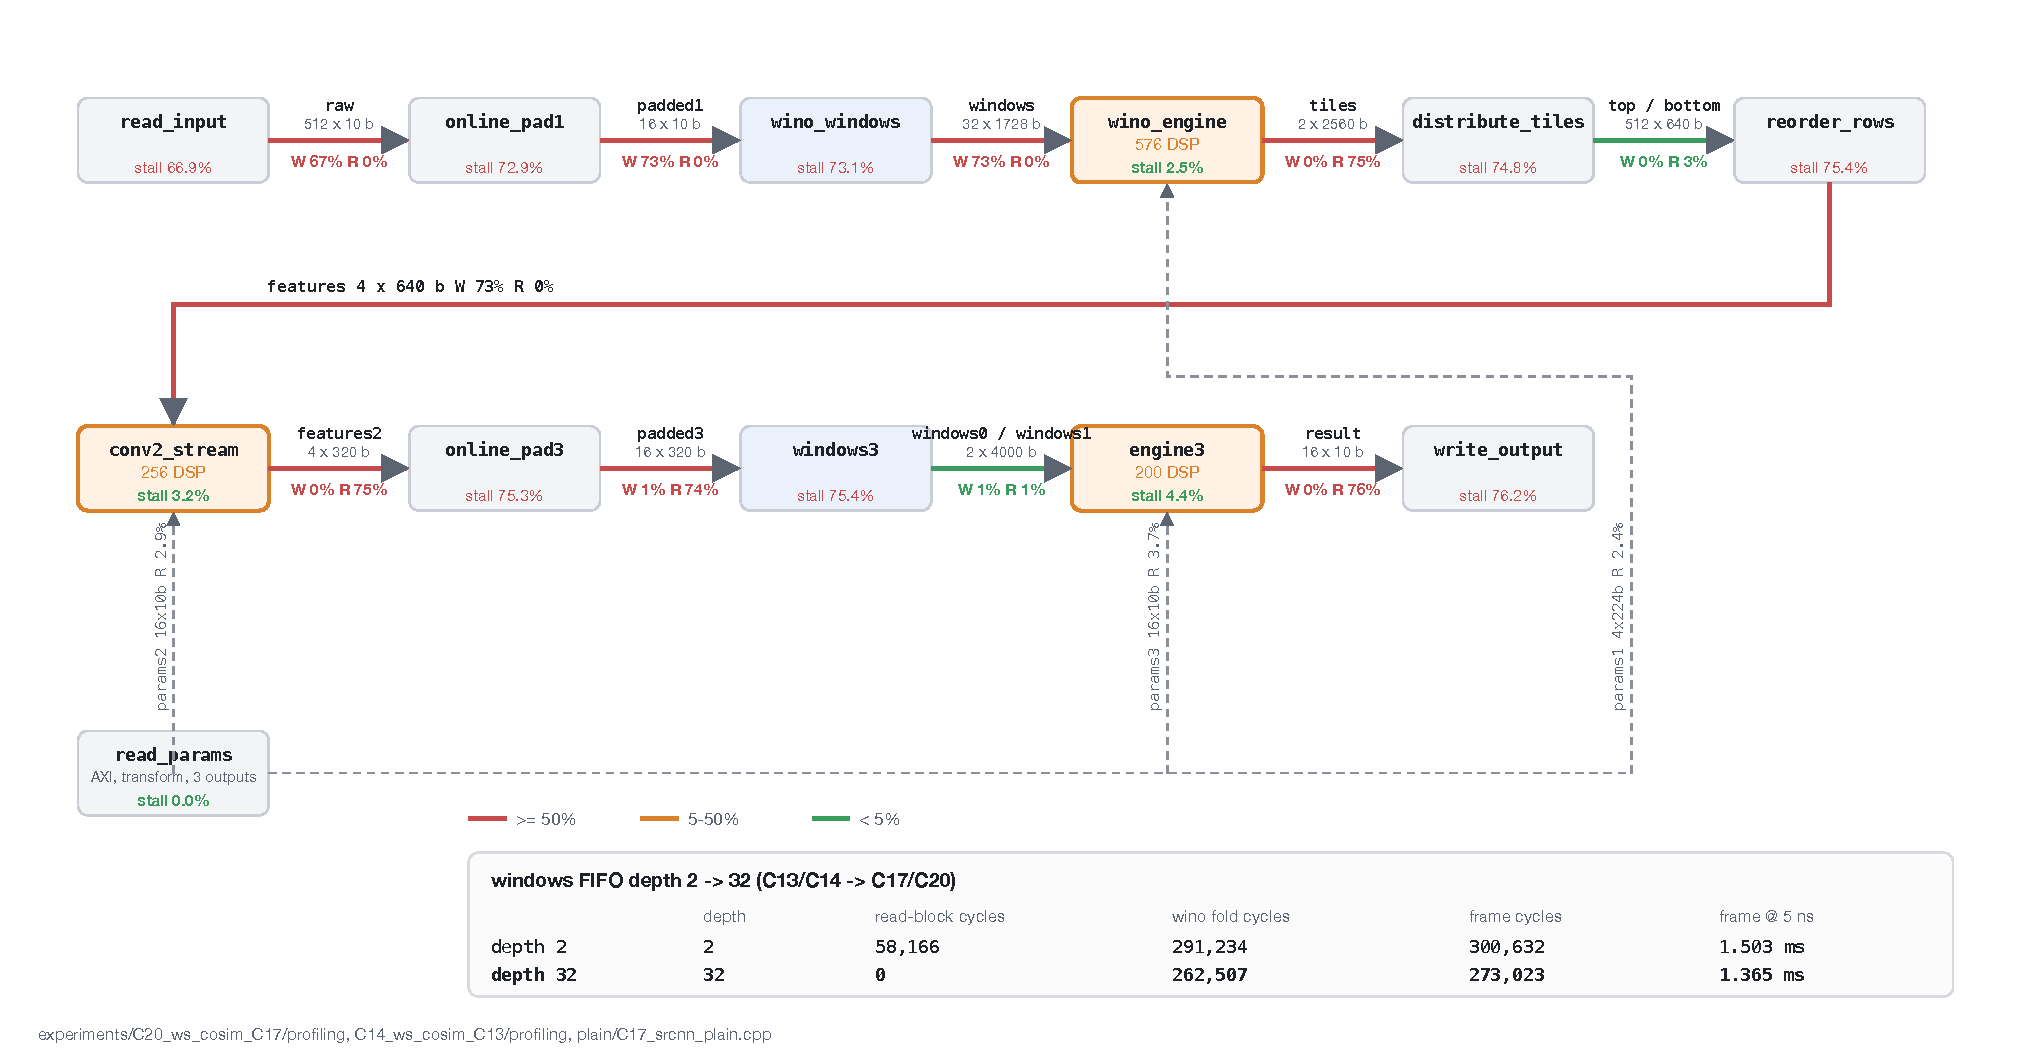
\includegraphics[width=\linewidth]{figures/fig04-dataflow-backpressure.pdf}
\caption{The dataflow region of the selected design: processes, FIFOs (depth $\times$ width in bits) and measured blocking from C/RTL co-simulation C20 over two frames. W / R is the share of cycles in which the FIFO blocked a write / a read; stall is the share of cycles in which the process waited. Inset: effect of the window FIFO depth, C14 (depth 2) against C20 (depth 32).}
\label{fig:4}
\end{figure}

\subsection{Resource allocation and optimisation for each layer}\label{sec:4.2}

MACs measure the amount of computation: to compute one output channel, every position in the K$\times$K window and every input channel is multiplied by a weight and accumulated, which is K$\times$K$\times$Cin operations; there are Cout output channels, so \textbf{MAC / output pixel = K $\times$ K $\times$ Cin $\times$ Cout.} Table~\ref{tab:4} gives the expected result for the three layers without any method magic.

\begin{table}[!htbp]
\centering
\footnotesize
\caption{Multiply-accumulate operations per output pixel for each layer of SRCNN and its share of the total.}
\label{tab:4}
\begin{tabular}{lllrr}
\toprule
Layer & Kernel & Channels & MAC / output pixel & Share \\
\midrule
conv1 & 9$\times$9 & 1$\rightarrow$64 & 5184 & 64.5\% \\
conv2 & 1$\times$1 & 64$\rightarrow$32 & 2048 & 25.5\% \\
conv3 & 5$\times$5 & 32$\rightarrow$1 & 800 & 10\% \\
\bottomrule
\end{tabular}
\end{table}

MACs decide resources. Building a multiplier out of logic is expensive on an FPGA, but the device provides DSP slices for exactly this, so we bind every multiplication to one DSP48E2 (one product per DSP per cycle; packing, which fits two, is introduced later). We then introduce the fold factor T: the number of clock cycles an engine spends on one output pixel. A layer with MAC multiplications per pixel takes T cycles per pixel, but needs only MAC/T multipliers, so T trades time for DSPs. The device has 1,248 DSP48E2 slices, so the task is to choose the smallest T whose DSP demand still fits, which is also the T that uses the device most fully.

At T = 4, direct conv1 alone needs 1,296 DSPs, more than the device has, and even Winograd conv1 with direct conv2 still needs 1,288. T = 4 becomes feasible only when both techniques are used together: Winograd on conv1 and packing on conv2, with conv3 small enough to stay direct (1,032 DSPs). T = 8 and T = 16 fit easily but double and quadruple the frame time, and T = 2 is out of reach with any combination. So T = 4 is the fastest fold that fits, and it is the row of Table~\ref{tab:5} where the two reductions are necessary rather than merely helpful.

\begin{table}[!htbp]
\centering
\footnotesize
\caption{DSPs needed per layer as a function of the fold T (cycles per output pixel), for the direct algorithm and for the selected reductions. Products per pixel: conv1 direct 5,184, conv1 Winograd 2,304; conv2 direct 2,048, conv2 packed 1,024 DSP-equivalents; conv3 800. The device limit is 1,248. The last column is the DSP count measured in synthesis for the experiments that implemented that row.}
\label{tab:5}
\begin{tabularx}{\linewidth}{cC{1.15cm}C{1.25cm}C{1.15cm}C{1.25cm}C{1.15cm}C{1.3cm}C{1.4cm}C{1.5cm}Y}
\toprule
T & conv1 direct & conv1 Winograd & conv2 direct & conv2 packed & conv3 direct & Total, all direct & Total, Winograd only & Total, Winograd + packing & Measured \\
\midrule
1 & 5,184 & 2,304 & 2,048 & 1,024 & 800 & 8,032 & 5,152 & 4,128 & -- \\
2 & 2,592 & 1,152 & 1,024 & 512 & 400 & 4,016 & 2,576 & 2,064 & -- \\
\textbf{4} & 1,296 & 576 & 512 & 256 & 200 & \textbf{2,008} & \textbf{1,288} & \textbf{1,032} & C13/C17: 1,032 \\
8 & 648 & 288 & 256 & 128 & 100 & 1,004 & 644 & 516 & F29/F30: 1,004; W21: 644; C10: 520 \\
16 & 324 & 144 & 128 & 64 & 50 & 502 & 326 & 258 & W18: 326 \\
\bottomrule
\end{tabularx}
\end{table}

The outcome of this allocation is shown in Table~\ref{tab:6}. After Winograd the three layers need 151 M, 133 M and 52 M multiplications per frame; with 576, 256 (each computing two products) and 200 DSPs, every layer needs 4 cycles per output pixel, a design bound of 4 $\times$ 255 $\times$ 255 = 260,100 cycles per frame. The C/RTL co-simulation C20 measured the three fold loops at 262,507, 260,877 and 261,885 cycles, within 1 \% of the bound and of each other. Because the stages run concurrently in a dataflow pipeline, the frame time is set by the slowest stage; the measurement confirms that no layer waits for another.

\begin{table}[!htbp]
\centering
\footnotesize
\caption{Fold-loop cycles per frame for the three engines: the design bound (loop trip count from the source) against the latency measured in C/RTL co-simulation C20. conv1 is bounded at 262,144 rather than 260,100 because its 2$\times$2 tiles cover a 256$\times$256 padded image.}
\label{tab:6}
\begin{tabular}{lrrr}
\toprule
layer & theory lower bound & C/RTL co-simulation & extra \\
\midrule
conv1(with edge padding) & 262,144 & 262,507 & +0.14 \% \\
conv2 & 260,100 & 260,877 & +0.30 \% \\
conv3 & 260,100 & 261,885 & +0.69 \% \\
\bottomrule
\end{tabular}
\end{table}

\subsection{Conv1: Winograd on nine 3$\times$3 sub-kernels}\label{sec:4.3}

\subsubsection{Principle}\label{sec:4.3.1}

Multiplication is expensive on an FPGA because it consumes DSPs, which are scarce; addition goes to LUTs, which are far cheaper. In the first layer, each output pixel needs the 9$\times$9 window of input pixels around it, for each of 64 output channels. But the windows of neighbouring output pixels obviously overlap, and the direct method still recomputes everything for each of them.

The smallest case, F(2,3), computes two outputs of a 3-tap filter from four inputs with 4 multiplications instead of 6:

\begin{lstlisting}[language={}]
# directly
y0 = d0·g0 + d1·g1 + d2·g2
y1 = d1·g0 + d2·g1 + d3·g2

# winograd: 
m1 = (d0 - d2) · g0
m2 = (d1 + d2) · (g0 + g1 + g2)/2
m3 = (d2 - d1) · (g0 - g1 + g2)/2
m4 = (d1 - d3) · g2

y0 = m1 + m2 + m3
y1 = m2 - m3 - m4
\end{lstlisting}

\subsubsection{Winograd on FPGA}\label{sec:4.3.2}

A very important property was utilized, which is that, for \textbf{multiplications or divisions that ever appear are $\times$2, $\times$\textonehalf{} and $\times$4, on FPGA those are binary shifts, which are fast and essentially free.}

The weight-side terms (g0 + g1 + g2)/2 are computed once when the weights are loaded; the input-side terms d0 $-$ d2 and the output sums are additions, which go to LUTs. The 2-D form F(2$\times$2, 3$\times$3) applies the same transforms along rows and columns: a 4$\times$4 input tile is transformed (B\textsuperscript{T} d B), multiplied element-wise by the transformed 3$\times$3 kernel (G g G\textsuperscript{T}), and the 4$\times$4 product is transformed back (A\textsuperscript{T} m A) to a 2$\times$2 output tile. That is 16 multiplications instead of 36 per 2$\times$2 tile, 2.25$\times$ fewer.

In integer arithmetic the \textonehalf{} in G is a division, which drops the lowest bit, and the Winograd result would no longer match the direct convolution. The fix is to use 2G instead of G, so the matrix becomes integer. In two dimensions the weight transform is U = (2G)$\cdot$g$\cdot$(2G)\textsuperscript{T}, which is the true U scaled by 4. Every later operation, the input transform, the element-wise products, the sum over the nine sub-blocks and the output transform, is then an integer add or multiply with no rounding, so the number that comes out is exactly 4 times the direct integer convolution result, its two lowest bits are always zero, and a right shift by 2 restores it bit for bit.

The transforms do widen the operands. Each transformed input value is a sum or difference of up to four pixels, so 10 bits become 12; each transformed weight is a sum of up to nine weights scaled by 2, so 10 bits become 14. The DSP48E2 multiplier is 27 $\times$ 18 bits, so a 12 $\times$ 14-bit product fits in one DSP, and each of the 16 products per tile costs exactly one DSP. The same widths are also why conv1 cannot use the two-products-per-DSP packing of conv2: two 14-bit weights at the 18-bit spacing that packing needs would occupy 32 bits, more than the 27-bit port, and the low-field product 12 $\times$ 14 = 26 bits would overflow the 18-bit field anyway. Winograd and packing are therefore not combined on the same layer; conv1 gets Winograd, conv2 gets packing.

\subsubsection{Why nine 3$\times$3 sub-kernels rather than a bigger tile.}\label{sec:4.3.3}

The 9$\times$9 kernel is cut into a 3$\times$3 grid of 3$\times$3 sub-kernels (the \texttt{group} index in the code). A 9-tap convolution is the sum of three 3-tap convolutions applied to the input at offsets 0, 3 and 6, and in two dimensions the 9$\times$9 convolution is the sum of nine 3$\times$3 convolutions at offsets (3a, 3b); nothing is approximated by the split. Each of the nine 3$\times$3 convolutions is then computed with Winograd F(2$\times$2, 3$\times$3), which produces a 2$\times$2 block of outputs from a 4$\times$4 block of inputs with 16 multiplications instead of 36. The 2$\times$2 output tile therefore needs a 10$\times$10 input window (2 + 9 $-$ 1 in each direction), and sub-kernel (a, b) reads the 4$\times$4 sub-block of that window starting at row 3a and column 3b; neighbouring sub-blocks share one row or column because a 3$\times$3 kernel on a 2$\times$2 tile needs 4$\times$4 input. The nine 4$\times$4 products are added in the transformed domain and the output transform runs once on the sum, which is valid because the transform is linear. One tile costs 9 $\times$ 16 = 144 multiplications for 4 pixels, 36 per pixel against 81 direct, a 2.25$\times$ reduction.

Working in 2$\times$2 tiles has a price downstream. The engine emits one tile every 16 cycles, but conv2 consumes pixels in raster order, so two processes after the engine (\texttt{distribute\_tiles}, \texttt{reorder\_rows}) split each tile into its upper and lower pixel pair and interleave even and odd rows back into scan order. Holding the odd rows until the even rows have gone out takes two 512-deep, 640-bit FIFOs, 36 BRAM18K, which is the largest memory cost of this layer, larger than the 9-row line buffer itself (9 BRAM18K). The padded image is also made 264$\times$264 instead of 263$\times$263 so that 128 $\times$ 128 tiles cover it exactly; the extra output row and column are discarded.

The tile size is a free parameter of Winograd: F(m, 3) computes m outputs per 1-D tile for any m, and m = 255 would process a whole image row at once. Larger tiles save more multiplications (per output pixel, ((m + 2)/m)\textsuperscript{2} against 9: 4 for m = 2, 2.25 for m = 4, approaching 1), so the question is why m = 2 is used. The answer is the transform constants, and multiplications cost . F(m, r) is built from polynomial interpolation at m + r $-$ 1 points; for m = 2 those are 0, 1, $-$1 and $\infty$, and the resulting matrices contain only 0, $\pm$1 and \textonehalf{}, which is why multiplying G by 2 makes everything integer and a 2-bit shift restores the result exactly. For m = 4 the interpolation needs six points (adding $\pm$2), and G contains 1/4, 1/6, 1/12 and 1/24: the smallest integer scaling is 24 per dimension, the result comes out 576 times too large, and dividing by 576 is no longer a shift. Besides, the transformed window is streamed as one element every T cycles, and its width is 9 sub-blocks $\times$ (m + 2)\textsuperscript{2} values $\times$ the transformed width: 1,728 bits for m = 2, but about 5,500 bits for m = 4 (36 values per sub-block, 17-bit operands), above the 4,096-bit aggregate stream limit of Vitis HLS that C09 ran into. Finally, a smaller conv1 would not shorten the frame on its own: with m = 4 conv1 needs 324 DSPs instead of 576 at T = 4, but the frame time is set by T, and moving the whole network to T = 2 fails on conv2 and conv3 regardless. Table~\ref{tab:7} collects the options. F(2$\times$2, 3$\times$3) is the only tile that is exact with shifts, nine of them cover the 9$\times$9 kernel without padding, and it is the one that was built and measured.

\begin{table}[!htbp]
\centering
\footnotesize
\caption{Options for conv1 at T = 4. Only the first two were synthesised; the F(4$\times$4, 3$\times$3) row is a paper estimate and was not pursued for the reasons in the text.}
\label{tab:7}
\begin{tabularx}{\linewidth}{YR{1.6cm}R{1.5cm}L{2.2cm}L{2.6cm}L{2.0cm}}
\toprule
Algorithm & Products per output pixel (64 ch) & DSPs at T = 4 & Transform constants & Exact with integer shifts & Window stream width \\
\midrule
Direct 9$\times$9 & 5,184 & 1,296 (> 1,248) & -- & yes & 10 b pixel \\
Nine 3$\times$3 sub-kernels, F(2$\times$2, 3$\times$3) \textbf{(selected)} & 2,304 & 576 & 1, \textonehalf{} & yes (G $\times$ 2, result >> 2) & 1,728 b \\
Nine 3$\times$3 sub-kernels, F(4$\times$4, 3$\times$3) & 1,296 & 324 & 1, \textonehalf{}, \textonequarter{}, 1/6, 1/12, 1/24 & no (scale 24\textsuperscript{2}, division by 9 remains) & $\approx$ 5,500 b (> 4,096 limit) \\
\bottomrule
\end{tabularx}
\end{table}

\textbf{Pipeline.} The layer is four processes (Table~\ref{tab:3}). \texttt{wino\_windows} slides a 10$\times$10 window over the padded 264$\times$264 image with a 9-row line buffer, and every second row and column emits the nine transformed 4$\times$4 sub-blocks as one 1,728-bit element. \texttt{wino\_engine} spends 16 cycles per window: in each cycle 4 output channels (4 lanes $\times$ 9 sub-blocks $\times$ 16 taps = 576 DSP products) are accumulated in the transformed domain, output-transformed, shifted, biased, and passed through ReLU and the round-to-10-bit quantiser; the 64 channels of the 2$\times$2 tile are collected in a shift register and written after cycle 15. \texttt{distribute\_tiles} and \texttt{reorder\_rows} turn tiles back into raster order and drop the extra row and column that the padding added so that 2$\times$2 tiles cover 255 pixels.

\subsection{conv2: two output channels per DSP}\label{sec:4.4}

\textbf{Budget.} conv2 is 25.5 \% of the MACs: 64 input channels $\times$ 32 output channels = 2,048 products per pixel, 512 DSPs at T = 4. The layer has 32 output channels but a 1$\times$1 kernel, so there is no spatial overlap to exploit and Winograd does not apply. Its DSP count still has to come down: with Winograd on conv1 and direct conv2 the network needs 1,288 DSPs, more than the 1,248 on the device.

\begin{figure}[!htbp]
\centering
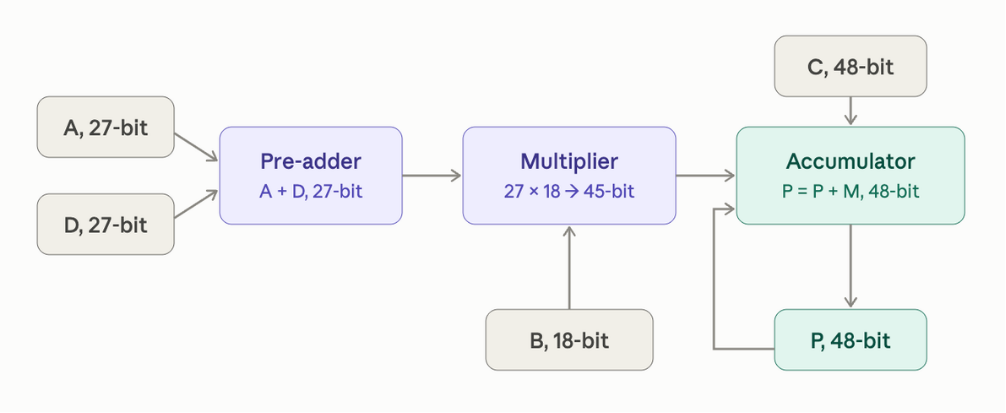
\includegraphics[width=0.8\figw]{figures/fig05-dsp48e2.png}
\caption{The DSP48E2 slice used for every multiplication in the design: a 27-bit pre-adder, a 27 $\times$ 18-bit signed multiplier and a 48-bit accumulator. conv2 packing places two 8-bit weights in the 27-bit A operand and the activation in the 18-bit B operand, so one multiplier yields two products; the pre-adder and accumulator are not used, because the sums are formed in fabric adder trees.}
\label{fig:5}
\end{figure}

\textbf{Principle.} A DSP48E2 multiplies a 27-bit by an 18-bit signed operand. The conv2 operands are a 10-bit activation and an 8-bit weight, so most of the 27-bit port is unused. Two weights for two output channels, w0 and w1, which share the same input activation x, are placed in one 27-bit word with a gap of 18 bits, \texttt{packed = w0 $\times$ 2\^{}18 + w1}. The single product is then

\begin{equation}
\text{packed} \times x = (w_0 \times x) \times 2^{18} + (w_1 \times x)
\end{equation}

A 10-bit activation times an 8-bit weight needs at most 17 bits plus a sign, so w1 $\times$ x stays inside the low 18 bits and never reaches the field of the second weight at bit 18 and above. Signs need no special arithmetic either: a negative w1 $\times$ x simply appears in the low field in two's complement, and because the packed word was formed as the integer w0 $\times$ 2\^{}18 + w1 (a negative w1 has already borrowed one from the w0 field), the DSP performs an ordinary integer multiplication. The only correction is at readout: when the low field is negative (bit 17 set) the high field reads w0 $\times$ x $-$ 1, and the engine adds the 1 back.

The packing itself is done once per frame when the weights are loaded (2,192 cycles), so no packing arithmetic runs per pixel; what remains per pixel is the borrow repair and the adder trees.

Why 8-bit weights are acceptable here is answered by the precision scan in Table~\ref{tab:8}. The smallest uniform precision that passes the $-$0.1 dB gate is 10-bit weights with 10-bit activations; uniform 8-bit weights lose about 5 dB. Quantizing only conv2 to 8-bit weights, however, passes: it costs 0.006 dB more than the uniform 10-bit point. There was also a way to pack without giving up 10-bit weights: the agent first split each weight into an 8-bit low part and a residual that is corrected after the multiplication (P07: exact, 1 DSP per pair, but 454 LUTs instead of 132). Applied to the whole network that costs 292,000 LUTs at T = 4 (P12), 2.5$\times$ the device, so conv2 carries 8-bit weights and a 21-bit accumulator while conv1 and conv3 keep 10-bit weights and are not packed.

\begin{table}[!htbp]
\centering
\footnotesize
\caption{Mean PSNR change of the fixed-point network against the float golden output over 13 images, from the precision scan E010 and the mixed-precision runs E062/E065. The gate for a design to be ranked was $-$0.1 dB.}
\label{tab:8}
\begin{tabular}{lrrll}
\toprule
Weights & Activations & $\Delta$PSNR (dB) & Worst image (dB) & Passes $-$0.1 dB gate \\
\midrule
16 & 10 & $-$0.046 & $-$0.171 & yes \\
10 & 10 & $-$0.070 & $-$0.226 & yes \\
10 & 8 & $-$0.645 & $-$1.958 & no \\
8 & 10 & $-$4.955 & $-$11.84 & no \\
8 & 8 & $-$5.180 & $-$12.14 & no \\
\textbf{10, conv2 only 8 (selected)} & \textbf{10} & \textbf{$-$0.076} & \textbf{$-$0.268 (foreman)} & \textbf{yes} \\
\bottomrule
\end{tabular}
\end{table}

\textbf{Pipeline.} \texttt{conv2\_stream} is one II = 1 loop that spends 4 cycles per pixel. In each cycle four lanes each take one channel pair: 64 packed multiplies, 64 borrow repairs, two 64-input adder trees (6 fabric levels, one register each), bias, truncation to 21 bits, ReLU and rounding to 10 bits; the 8 channels per cycle are collected in a shift register and the 32-channel pixel is written after cycle 3. Per cycle that is 256 DSPs producing 512 products. The widths along the path are: 37-bit product, 23-bit sums, 21-bit accumulator before ReLU, 10-bit output with 7 fraction bits. The 21-bit truncation relies on the sum range, which the C simulation checks with an assertion over the test set.

\textbf{Cost.} HLS estimate: 256 DSPs, 37,074 LUTs, 80,091 FFs. Routed (C22): 256 DSPs, 16,009 LUTs, 17,759 FFs, no BRAM. The 2.3$\times$ LUT and 4.5$\times$ FF difference between estimate and routed result is the largest of the three layers and comes from the register-heavy adder trees that Vivado retimes.

\subsection{conv3: direct 5$\times$5 convolution, folded over four cycles}\label{sec:4.5}

\textbf{Budget.} conv3 is 10 \% of the MACs: 25 taps $\times$ 32 input channels = 800 products per output pixel, 200 DSPs at T = 4. Since the main step that limits the speed is not conv3, therefore, as long as conv3 can complete the task within T = 4 using limited resources, it will be sufficient.

\textbf{Principle.} The layer is a classic streaming convolution: a line buffer plus a sliding window. \texttt{windows3} keeps the last four rows of the padded 259$\times$259 feature map, 32 channels of 10 bits each, in BRAM (4 $\times$ 259 $\times$ 320 bits = 36 BRAM18K), and a 5$\times$5$\times$32 window in registers. Each incoming pixel shifts the window one column: the new column is the four stored rows plus the new pixel, and the line buffer shifts up one row at the same address. From the fifth row and column on, every pixel yields a complete window, so the stage emits 65,025 windows for 67,081 input pixels. The window is 8,000 bits and goes out as two 4,000-bit halves (channels 0 to 15 and 16 to 31) because of the 4,096-bit stream limit noted in the dataflow section.

\texttt{engine3} folds the 800 products over 4 cycles: in cycle k it multiplies input channels 8k to 8k+7 by all 25 taps (200 DSPs, 10 $\times$ 10 $\rightarrow$ 20 bits), zero-pads the 200 products to 256 and adds them in an 8-level fabric adder tree with one register per level, then adds the partial to a 23-bit running sum that starts from the bias in cycle 0. After cycle 3 the sum is rounded half to even to 10 bits with saturation and written out. There is no ReLU; the 10-bit integer is decoded to a float exactly by assembling the IEEE fields rather than by a float-conversion core. The pipeline depth of 13 cycles is mostly the adder tree; at II = 1 this depth is paid once per frame, not per pixel.

\begin{figure}[!htbp]
\centering
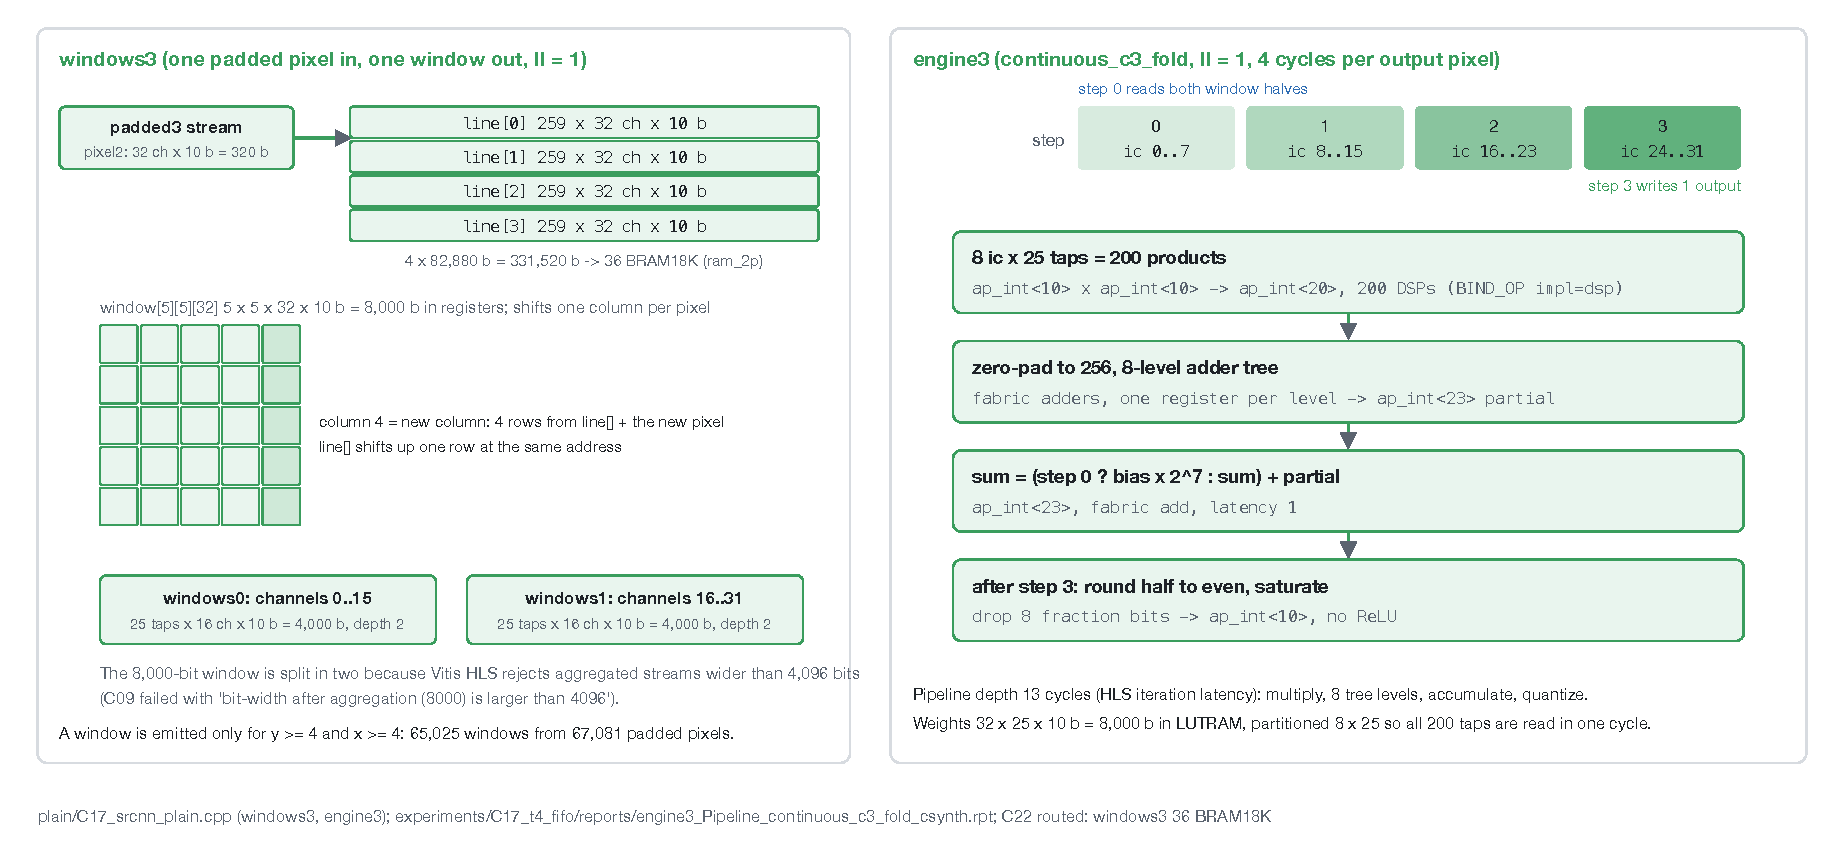
\includegraphics[width=\linewidth]{figures/fig06-conv3-window-engine.pdf}
\caption{conv3: window generation and folded engine. Left: four line-buffer rows and the 5$\times$5$\times$32 register window; the window leaves as two 4,000-bit halves. Right: the four-cycle fold, 200 DSP products and a 256-input adder tree per cycle, accumulated into a 23-bit sum.}
\label{fig:6}
\end{figure}

\textbf{Why it stays direct.} The alternatives were measured and rejected. A scatter formulation, which stores five rows of partial sums instead of four rows of input and adds each incoming pixel into the 25 outputs it affects, cuts conv3 BRAM from 36 to 5 blocks but costs 34 \% to 56 \% more cycles (G01 to G03, controlled comparison at T = 32), because it must visit every padded source pixel and prime and flush partial rows at every image edge; in this design BRAM is not scarce (38 \% used after routing) and cycles are, so the trade is the wrong way round. Packing two products per DSP needs 8-bit weights or a residual correction; with conv3's 10-bit weights the residual version synthesised to 260,882 LUTs, 2.2$\times$ the device (C05). Winograd on a 5$\times$5 kernel would need padding to 6$\times$6 and would save at most 72 DSPs, 6 \% of the device, for the same transform fabric that conv1 pays; it was not pursued.

\textbf{Cost.} HLS estimate: 200 DSPs, 36 BRAM18K, 29,835 LUTs, 53,879 FFs. Routed (C22): 200 DSPs, 36 BRAM18K, 13,515 LUTs, 48,418 FFs, of which the window generator is 3,248 LUTs and 17,692 FFs and the engine 10,243 LUTs and 14,705 FFs. The 36 BRAM18K line buffer is the single largest memory in the design after the two raster FIFOs of conv1.

\subsection{Sources for the numbers in this chapter}\label{sec:4.6}

Every number quoted in this chapter can be traced to a file in the project repository; Table~\ref{tab:9} lists them. Experiment IDs (W01, P07, C17, \ldots{}) are directories under \texttt{experiments/\allowbreak{}}, each holding the experiment card, the tool reports and the parsed metrics.

\begin{table}[!htbp]
\centering
\footnotesize
\caption{Source of every number quoted in this chapter, by file in the project repository.}
\label{tab:9}
\begin{tabularx}{\linewidth}{L{5.2cm}Y}
\toprule
Number & Source \\
\midrule
Stage widths, depths, loop bounds (Table~\ref{tab:3}) & \texttt{plain/\allowbreak{}C17\_\allowbreak{}srcnn\_\allowbreak{}plain.cpp}; FIFO instance names in \texttt{experiments/\allowbreak{}C22\_\allowbreak{}ws\_\allowbreak{}impl\_\allowbreak{}C17/\allowbreak{}physical\_\allowbreak{}hierarchy\_\allowbreak{}routed.csv} (\path{fifo_w1728_d32}, \path{fifo_w4000_d2}, \ldots{}) \\
Measured active cycles and stall (Table~\ref{tab:3}, Table~\ref{tab:6}, Figure~\ref{fig:4}) & \texttt{experiments/\allowbreak{}C20\_\allowbreak{}ws\_\allowbreak{}cosim\_\allowbreak{}C17/\allowbreak{}profiling/\allowbreak{}processes.csv}, \path{channels.csv} \\
Routed per-module LUT/FF/BRAM/DSP & \texttt{experiments/\allowbreak{}C22\_\allowbreak{}ws\_\allowbreak{}impl\_\allowbreak{}C17/\allowbreak{}physical\_\allowbreak{}hierarchy\_\allowbreak{}routed.csv} \\
HLS per-module estimates, pipeline depths 8/11/13 & \texttt{experiments/\allowbreak{}C17\_\allowbreak{}t4\_\allowbreak{}fifo/\allowbreak{}C17.md} (Module resources; Pipeline depth table) \\
DSP table rows (Table~\ref{tab:5}) & W18, F29, F30, W21, C10, C13, C17 metrics in \texttt{experiments/\allowbreak{}ARCH\_\allowbreak{}SUMMARY.md} \\
Winograd PE & \texttt{experiments/\allowbreak{}W01\_\allowbreak{}integer\_\allowbreak{}f2\_\allowbreak{}10bit}, \path{W02_direct_f2_control} \\
Packing PE & \texttt{experiments/\allowbreak{}P01\_\allowbreak{}signed8\_\allowbreak{}pair} (exhaustive), \path{P02_signed8_direct_control}, \path{P07_exact10_residual_pair}, \path{P12_exact10_packing_T4} \\
Prepacking at load & \texttt{experiments/\allowbreak{}C13\_\allowbreak{}runtime\_\allowbreak{}prepacked\_\allowbreak{}conv2\_\allowbreak{}T4/\allowbreak{}C13.md} \S{}6 \\
Precision scan (Table~\ref{tab:8}) & \texttt{experiments/\allowbreak{}E010\_\allowbreak{}precision\_\allowbreak{}scan/\allowbreak{}data.csv}; \path{E065_apfixed_mixed_conv2w8}; per-image values \texttt{experiments/\allowbreak{}C17\_\allowbreak{}t4\_\allowbreak{}fifo/\allowbreak{}quality.csv} \\
conv3 gather vs scatter & \texttt{experiments/\allowbreak{}conv3\_\allowbreak{}comparison.csv}; G01, G02, G03, E060 cards \\
conv3 packing attempt & \texttt{experiments/\allowbreak{}C05\_\allowbreak{}wino\_\allowbreak{}packing\_\allowbreak{}T4\_\allowbreak{}conv3\_\allowbreak{}header\_\allowbreak{}retry/\allowbreak{}C05.md} \\
4,096-bit stream limit & \texttt{experiments/\allowbreak{}C09\_\allowbreak{}wino\_\allowbreak{}conv2w8\_\allowbreak{}continuous\_\allowbreak{}T4/\allowbreak{}C09.md} (archived error) \\
\bottomrule
\end{tabularx}
\end{table}
